\documentclass{beamer}
\usepackage{times, amsthm, amsmath, amssymb, cancel, changepage, graphicx, lipsum, fancyhdr, mathabx, enumitem,caption, subcaption}
\usetheme{CambridgeUS}
\usecolortheme{seagull}
\usefonttheme{serif}
\definecolor{navy}{RGB}{0, 0, 128} 
\setbeamercolor{frametitle}{fg=navy}
\setbeamercolor{title}{fg=navy}
\setbeamerfont{frametitle}{series=\bfseries}
\setbeamerfont{title}{series=\bfseries}


\title{Lecture 5: Sequences \& Series I}
\date{September 10, 2019}

\begin{document}
	
\frame{\titlepage}

\begin{frame}
\frametitle{What is a Sequence?}
A sequence is a set of numbers written in some order
$$a_1, a_2, a_3,...,a_{n-1}, a_n$$
An infinite sequence can be thought of as a function whose domain is the set of positive integers $i \in \mathbb{I}$ such that
$$a_i = f(i)$$

\vspace{6pt}
\textbf{Examples:}\\
Give the first four terms of the following sequences
\begin{itemize}
	\item[(a)] $a_n = \frac{n}{n+1}$
	\item[(b)] $a_n = 2 + (.1)^n$
	\item[(c)] $a_n = (-1)^{n+1} \frac{n^2}{3n-1}$
	\item[(d)] $a_n = 4$
\end{itemize}
\end{frame}

\begin{frame}
\frametitle{Limits of Sequences}
A sequence $\{a_n\}$ has the limit
$$\lim\limits_{n \to \infty} \{a_n\} = L$$
if for all $\epsilon > 0$ there exits a positive $N$ such that $|a_n-L| < \epsilon$ whenever $n>N$. If the limit exists then the sequence converges, otherwise the sequence diverges.

\vspace{6pt}
\textbf{Examples:}\\
If possible, find the limit of the following sequences:
\begin{itemize}
	\item[(a)] $\{\frac{n}{2n+1}\}$
	\item[(b)] $\{ \frac{(-1)^nn^2}{1+n^3}\}$
	\item[(c)] $\{(1+\frac{c}{n})^n\}$
\end{itemize}
\end{frame}

\begin{frame}
\frametitle{What is a Series?}
If we add the terms of a sequence $\{a_n\}$ then we get an infinite series.
$$a_1+a_2+...+a_n+... = \sum_{i=1}^\infty a_i$$
If we add the first $n$ terms of a sequence, we get the $n^{th}$ partial sum.
\begin{eqnarray*}
	S_1 &=& a_1 \\
	S_2 &=& a_1 + a_2\\
	\vdots &=& \vdots\\
	S_n &=& a_1 +,...,+a_n
\end{eqnarray*}

If the sequence of partial sums $\{S_n\}$ converges and $\lim\limits_{n \to \infty}S_n=S$ then the series $\sum_{i=1}^{\infty} a_i$ is convergent. Otherwise  $\sum_{i=1}^{\infty} a_i$ is divergent.

Properties of infinite series can be found 
\end{frame}

\begin{frame}
\frametitle{Geometric Series}
The geometric series has the form
$$a + ar + ar^2 + ar^3 +... = \sum_{n=1}^\infty ar^{n-1} \mbox{ for } a\neq 0$$
For $|r|<1$ the geometric series $\sum_{n=1}^\infty ar^{n-1}$ converges and its sum is 
$$\sum_{n=1}^\infty ar^{n-1} =\frac{a}{1-r}$$

\vspace{6pt}
\textbf{Examples:}
\begin{itemize}
	\item[(a)] Find the sum of $\sum_{n=1}^\infty 2(\frac{3}{4})^{n-1}$
	\item[(b)] Is this convergent and find its sum: $4+\frac{8}{5} + \frac{16}{25} + \frac{32}{125} + ...$.
	\item[(c)] Find the sum of $\sum_{x=0}^\infty p(1-p)^x$
	\item[(d)] Does $\sum_{n=1}^\infty 2^{2n} 3^{1-n}$ converge?
\end{itemize}
\end{frame}

\begin{frame}
\frametitle{Limits and Convergence}

\begin{theorem}
	If the series $\sum_{n=1}^\infty a_n$ is convergent, then 
	$$\lim\limits_{n \to \infty} a_n = 0$$
	If the $\lim\limits_{n \to \infty} a_n$ does not exist or if $\lim\limits_{n \to \infty} a_n \neq 0$, then the series $\sum_{n=1}^\infty a_n$  is divergent.
\end{theorem}
Note: If $\lim\limits_{n\to \infty} a_n = 0$, this does not mean that $\sum_{n=1}^\infty a_n$ is convergent.

\vspace{12pt}
\textbf{Example:}
\begin{itemize}
	\item[(a)] Does $\sum_{n=1}^\infty \frac{1}{n}$ converge?
\end{itemize}
\end{frame}

\begin{frame}
\frametitle{Convergence Rules}
Let $\{a_n\}$ and $\{b_n\}$ be two sequences such that $\sum_{n=1}^\infty a_n$ converges to $A$ and $\sum_{n=1}^\infty b_n$ converges to $B$ and let $c$ be a constant. Then
\begin{itemize}
	\item[(i)] $\sum_{n=1}^\infty a_n \pm  \sum_{n=1}^\infty b_n = A \pm B$
	\item[(ii)] $\sum_{n=1}^\infty c a_n = cA$
	\item[(iii)] $(\sum_{n=1}^\infty a_n )(\sum_{n=1}^\infty b_n ) = AB$
\end{itemize}
\vspace{12pt}
\textbf{Examples:}
\begin{itemize}
	\item[(a)] Does $\sum_{n=1}^{\infty} (\frac{3}{n(n+1)} + \frac{1}{2^n})$ converge?
	\item[(b)] Coin flipping.
\end{itemize}
\end{frame}

\begin{frame}
\frametitle{Series With Positive Terms}

\end{frame}

\begin{frame}
\frametitle{Tests of Convergence: Integral Test}
\end{frame}

\begin{frame}
\frametitle{Tests of Convergence: Limit Comparison Test}
\end{frame}

\begin{frame}
\frametitle{Tests of Convergence: Ratio Test}
\end{frame}

\begin{frame}
\frametitle{Absolute Convergence}
\end{frame}

\begin{frame}
\frametitle{Power Series}
\end{frame}

\begin{frame}
\frametitle{Strategies for Testing Series}
\end{frame}

\begin{frame}
\frametitle{Taylor Series}
\end{frame}

\begin{frame}
\frametitle{Examples}
\end{frame}

%\begin{frame}
%\frametitle{What is a Limit?}
%\begin{figure}
%	\centering
%	\begin{subfigure}{0.48\textwidth}
%		
%		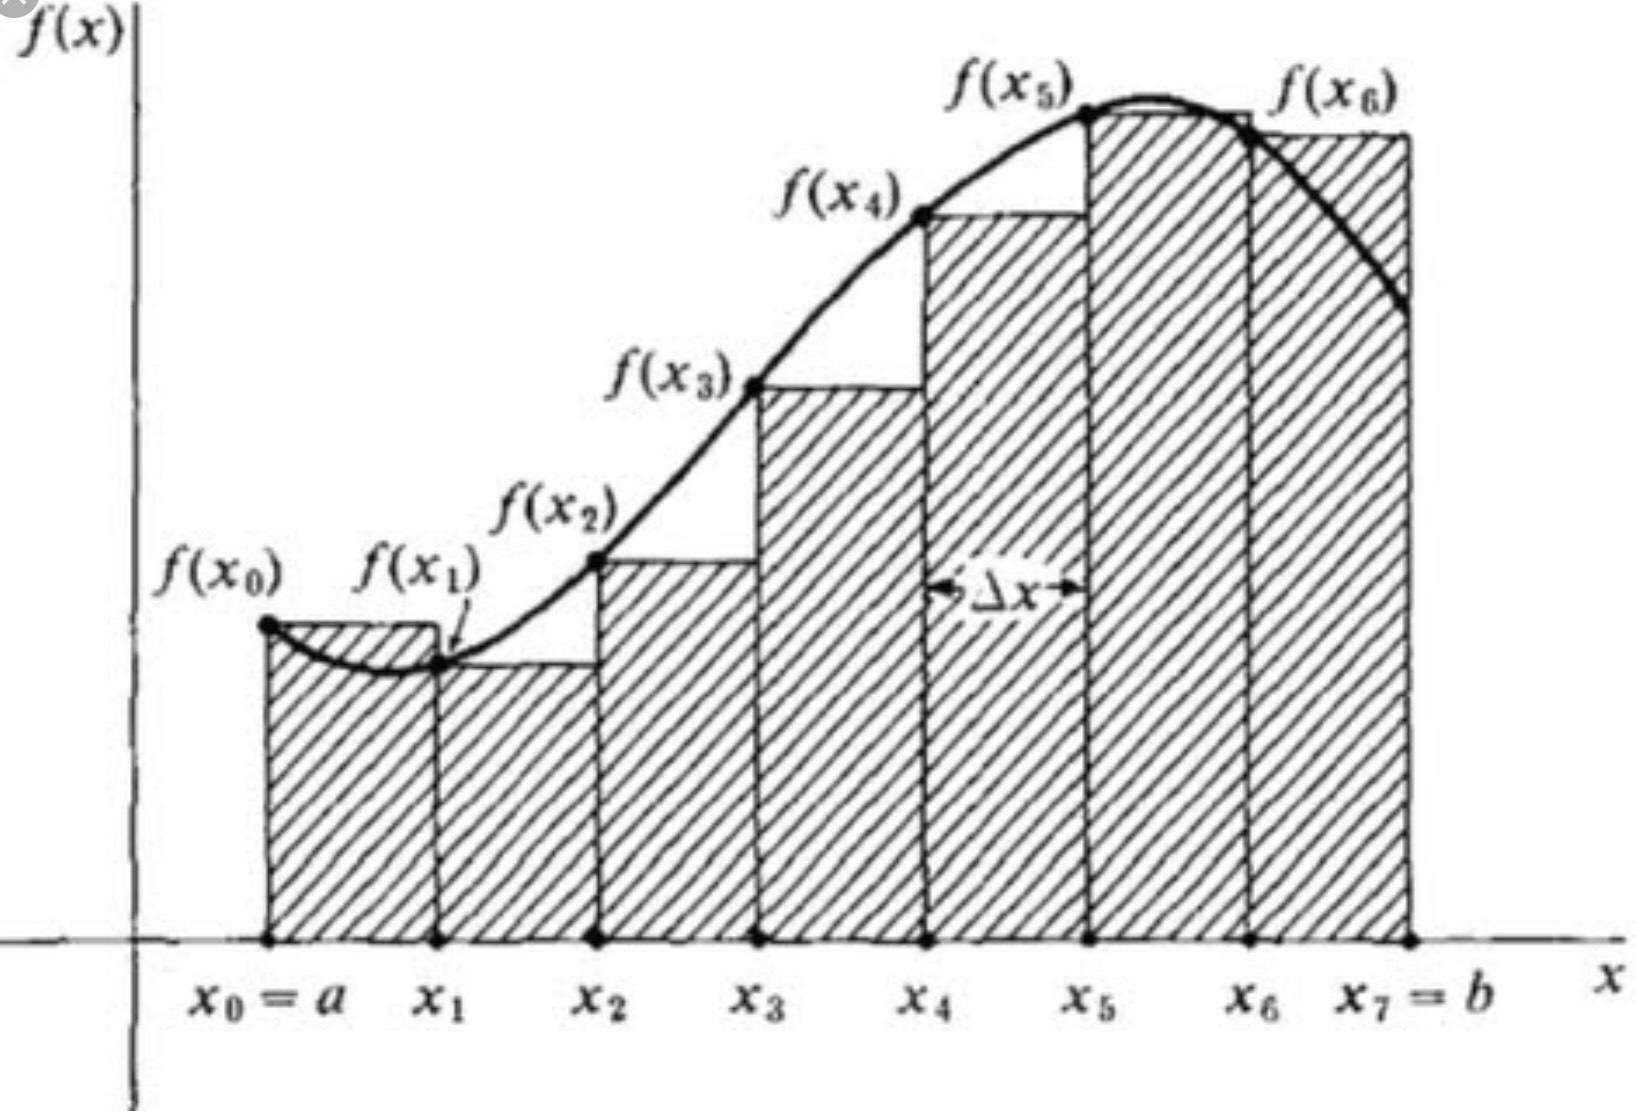
\includegraphics[width=\textwidth]{IMG_0380.jpg}
%		\hspace*{10pt}\hbox{\thinspace{\tiny\itshape vias.org}}
%		\caption{Single integration}
%	\end{subfigure}% 
%	~ 
%	\begin{subfigure}{0.48\textwidth}
%		
%		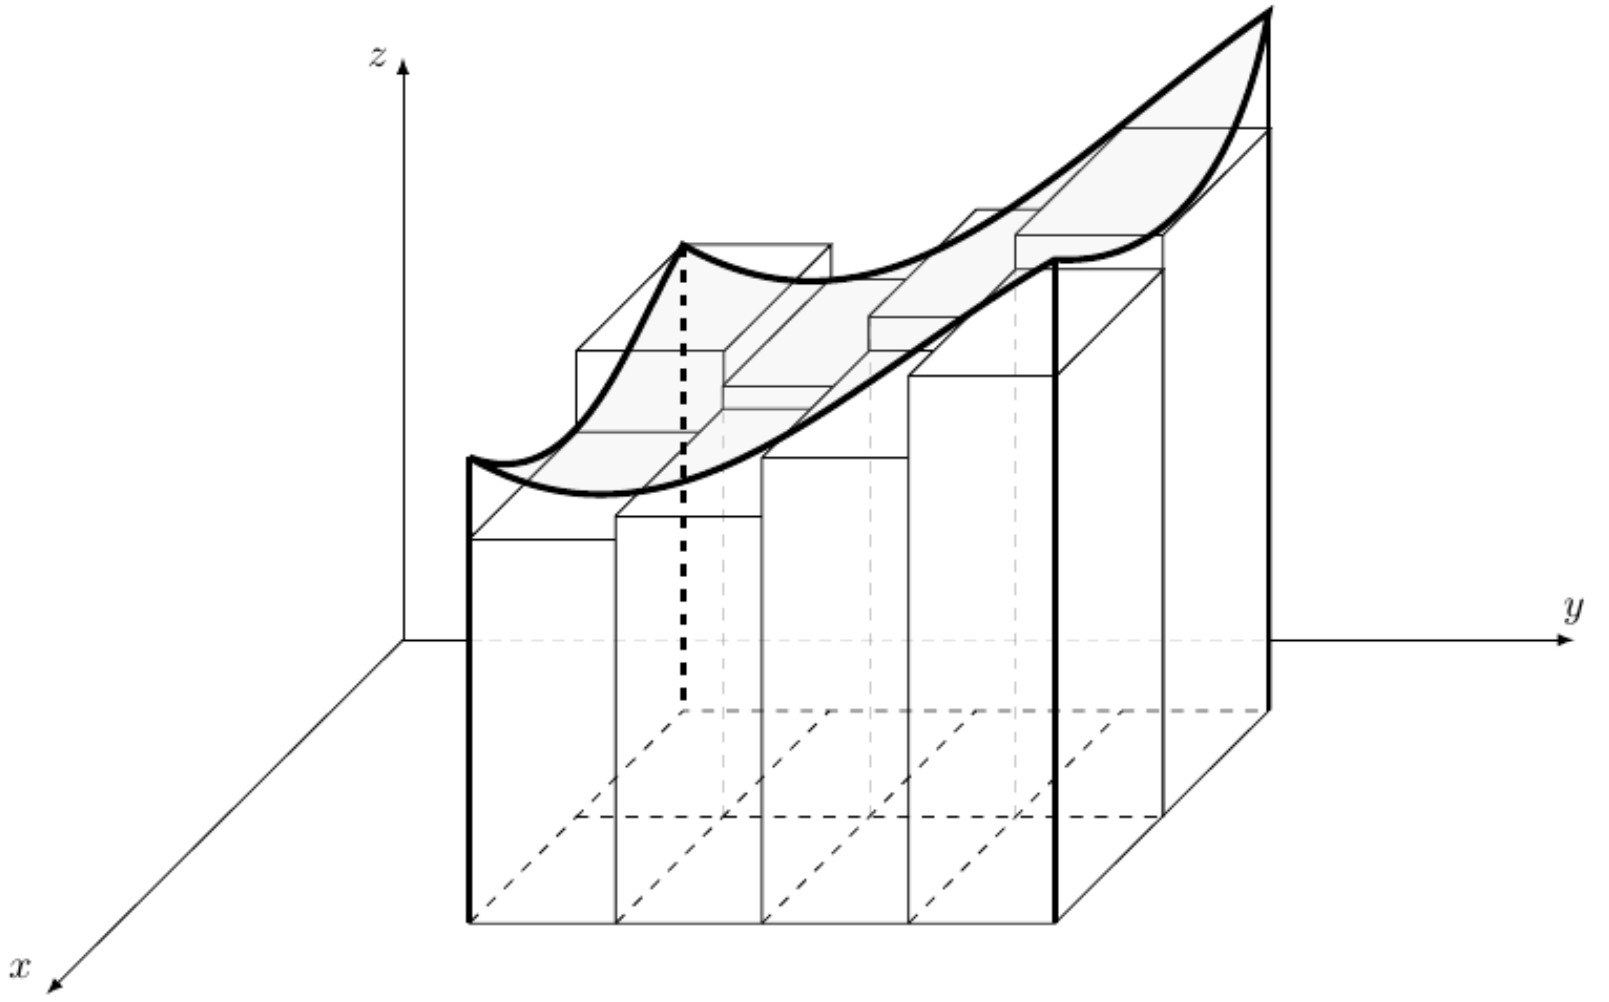
\includegraphics[width=\textwidth]{IMG_0385.jpg}
%		\hspace*{10pt}\hbox{\thinspace{\tiny\itshape tex.stackexchange.com}}
%		\caption{Double integration.}
%		\label{fig:2}
%	\end{subfigure}
%\end{figure}
%
%\end{frame}
%
%
%\begin{frame}
%\frametitle{Triple Integral}
%\begin{figure}
%	\centering
%	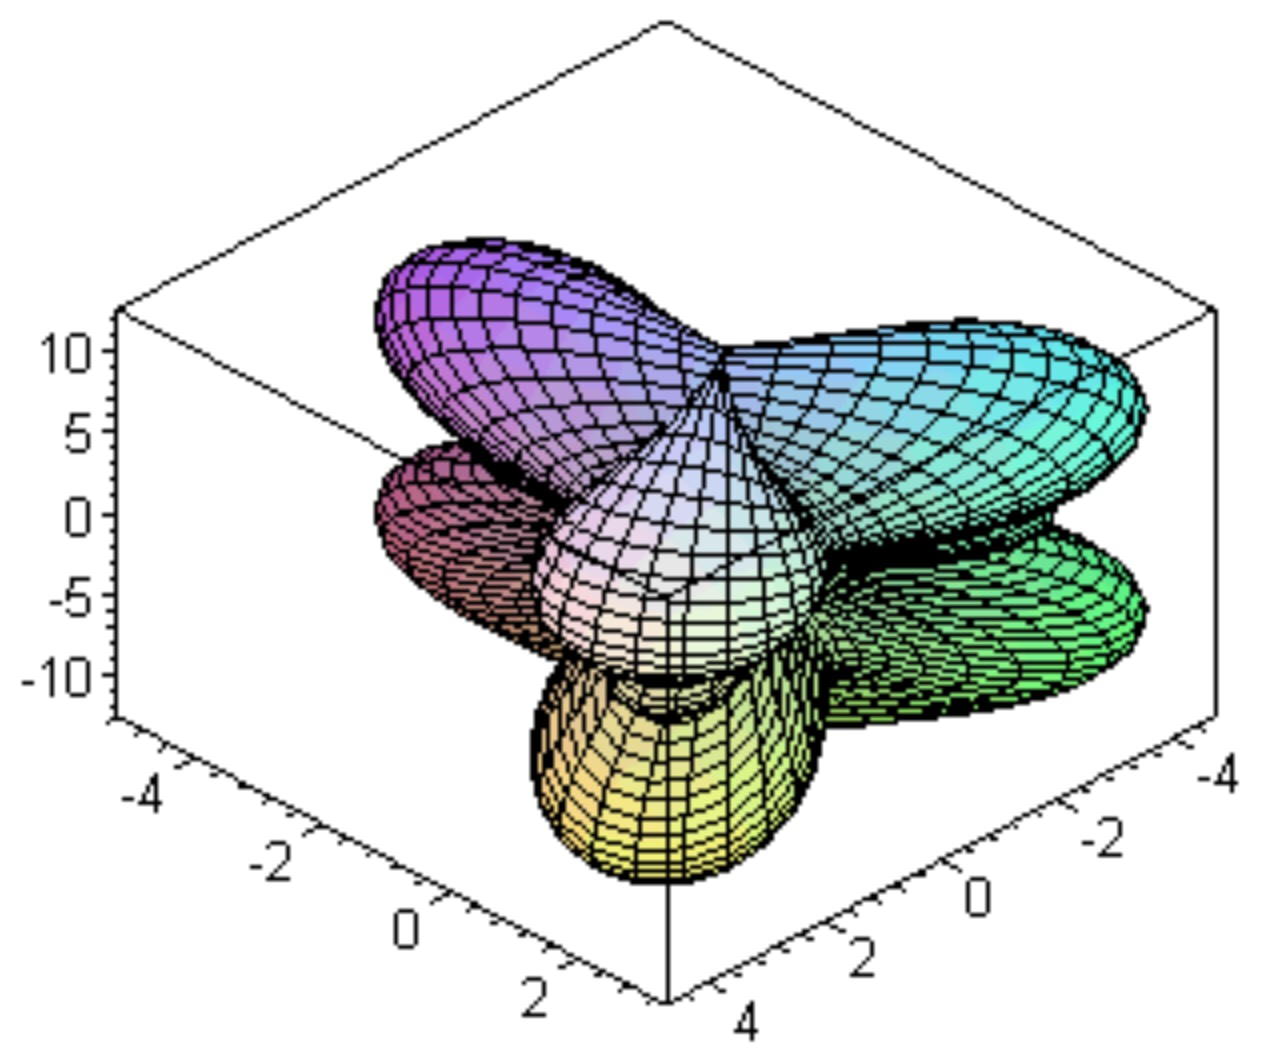
\includegraphics[height=.45\textheight]{IMG_0384.jpg}\\
%	\hspace*{10pt}\hbox{\thinspace{\tiny\itshape maplesoft.com}}
%\end{figure}
%
%$$\iiint\limits_{\mathbb{R}} F(x,y,z) dV = \int_{x=a}^{x=b} \int_{y=y_1(x)}^{y=y_2(x)} \int_{z=z_1(x,y)}^{z=z_2(x,y)} F(x,y,z) dz\,dy\,dx$$
%\textbf{Example:}
%\begin{itemize}
%	\item[(a)] $\int_0^1 \int_0^{1-x} \int_0^{2-x} xyz \,dz\,dy\,dx$
%\end{itemize}
%\end{frame}

\end{document}
